\documentclass[12pt, a4paper, numeric]{article}

\usepackage{setspace, a4wide}
\usepackage{filecontents, fancyhdr}
\usepackage[croatian]{babel}
\usepackage[utf8]{inputenc}
\usepackage{graphicx}
\usepackage{subcaption}
\usepackage{booktabs}
\usepackage{graphicx}
\usepackage{subcaption}
\usepackage{hyperref} 
\usepackage{commath}

\onehalfspacing
\pagestyle{fancy}
\fancyhf{}
\chead{Neizrazito, evolucijsko i neuro računarstvo}

\begin{document}
\pagebreak

\section*{1. zadatak}
Slika \ref{fig:zad1} prikazuje graf funkcije izlaza neurona tipa 1 s različitim parametrima $s$. 
Izlaz neurona definiran je kao:
\[
    y = \frac{1}{1 + \frac{|x - w|}{|s|}}.
\]
Vidljivo je kako promjena parametra $s$ rezultira promjenom širine funkcije, na način da manje vrijednosti $s$ određuju uže funkcije.
Za slučaj neurona sa $2$ ulaza funkcija bi bila šiljasto zvonolika u $3-$dimenzijskom prostoru.

\begin{figure}[ht!] 
    \centering
    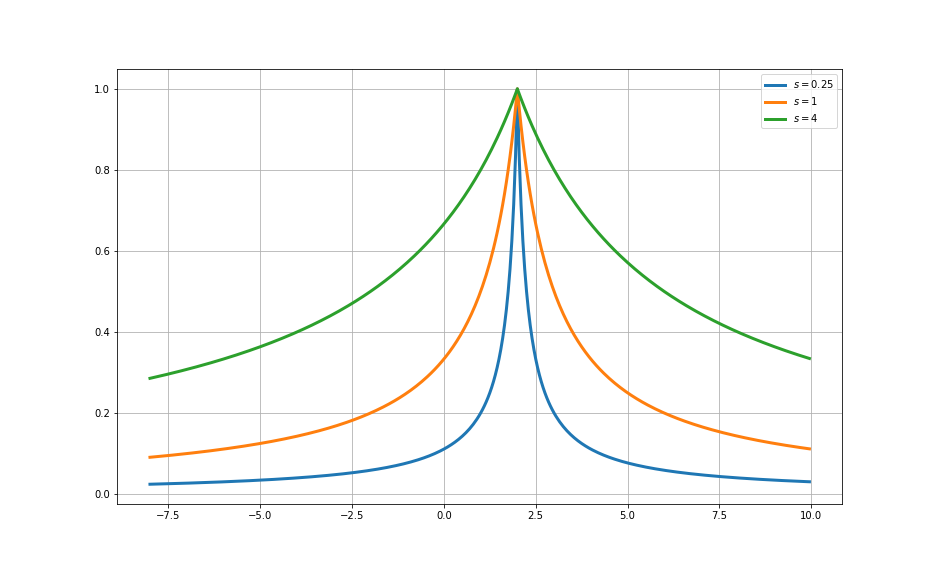
\includegraphics[width=1\textwidth]{img/zadatak1}
    \captionsetup{justification=centering}
    \caption{Prikaz izlaza neurona tipa 1 s različitim parametrima $s$}
    \label{fig:zad1}
\end{figure}
\pagebreak

\section*{2. zadatak}

\begin{figure}[ht!] 
    \centering
    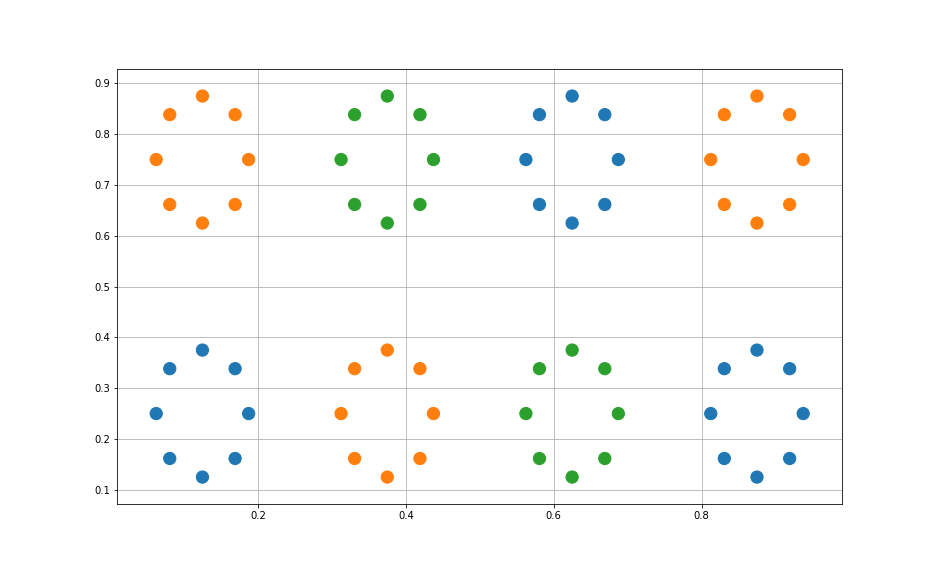
\includegraphics[width=1\textwidth]{img/zadatak2}
    \captionsetup{justification=centering}
    \caption{Prikaz podataka iz skupa za učenje}
    \label{fig:zad2}
\end{figure}
\pagebreak

\section*{3. zadatak}
\begin{figure}[ht!] 
    \centering
    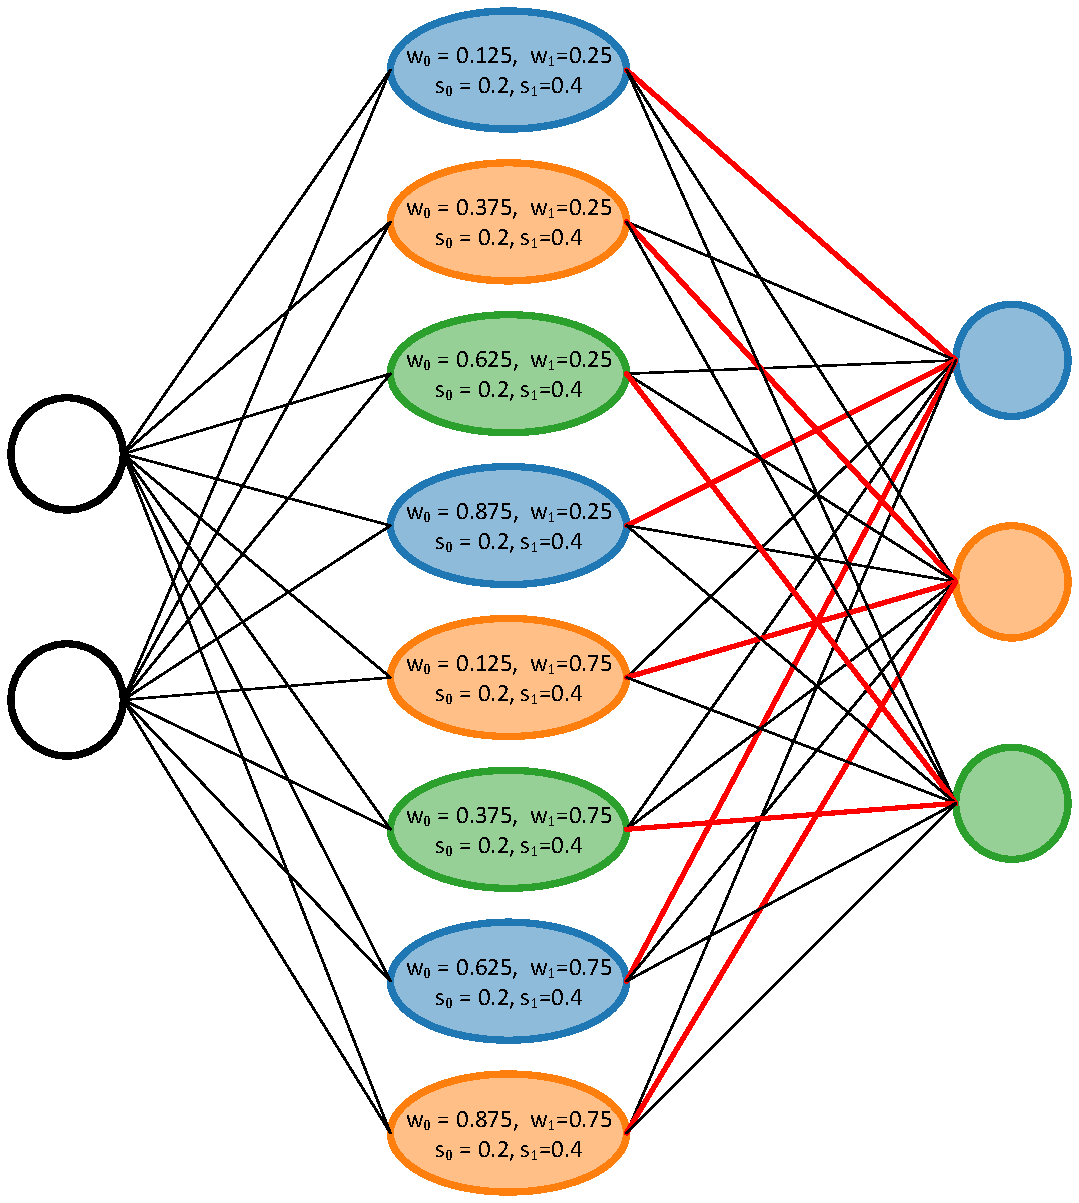
\includegraphics[width=0.9\textwidth]{img/neural}
    \captionsetup{justification=centering}
    \caption{Prijedlog težina neuronske mreže}
    \label{fig:zad3}
\end{figure}
Predložene težine za neurone skrivenog sloja upisane su unutar neurona te su određene na način da svaki neuron odgovara centroidu jedne grupe podataka.
Težine izlaznog sloja nisu upisane na slici već su vizualno prikazane bojama na način da crvene težine imaju veliku pozitivnu vrijednost (npr. $150$), dok crne težine imaju negativnu vrijednost koja je po apsolutnom iznosu $3$ puta manja od pozitivne (npr. $-50$).
\pagebreak

\section*{4. zadatak}
\begin{figure}[ht!] 
    \centering
    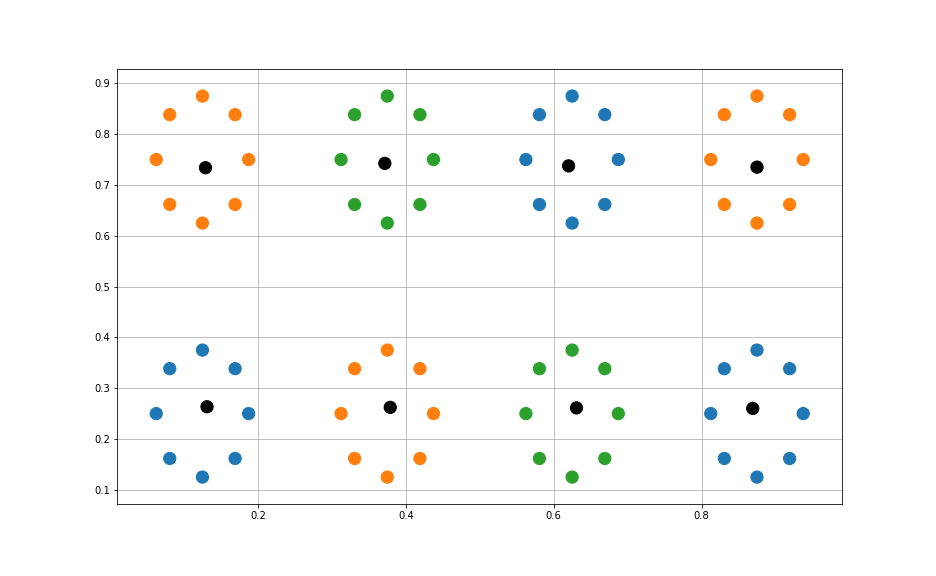
\includegraphics[width=1\textwidth]{img/zadatak4}
    \captionsetup{justification=centering}
    \caption{Centroidi dobiveni učenjem mreže arhitekture $2x8x3$}
    \label{fig:zad4}
\end{figure}
\begin{figure}[ht!] 
    \centering
    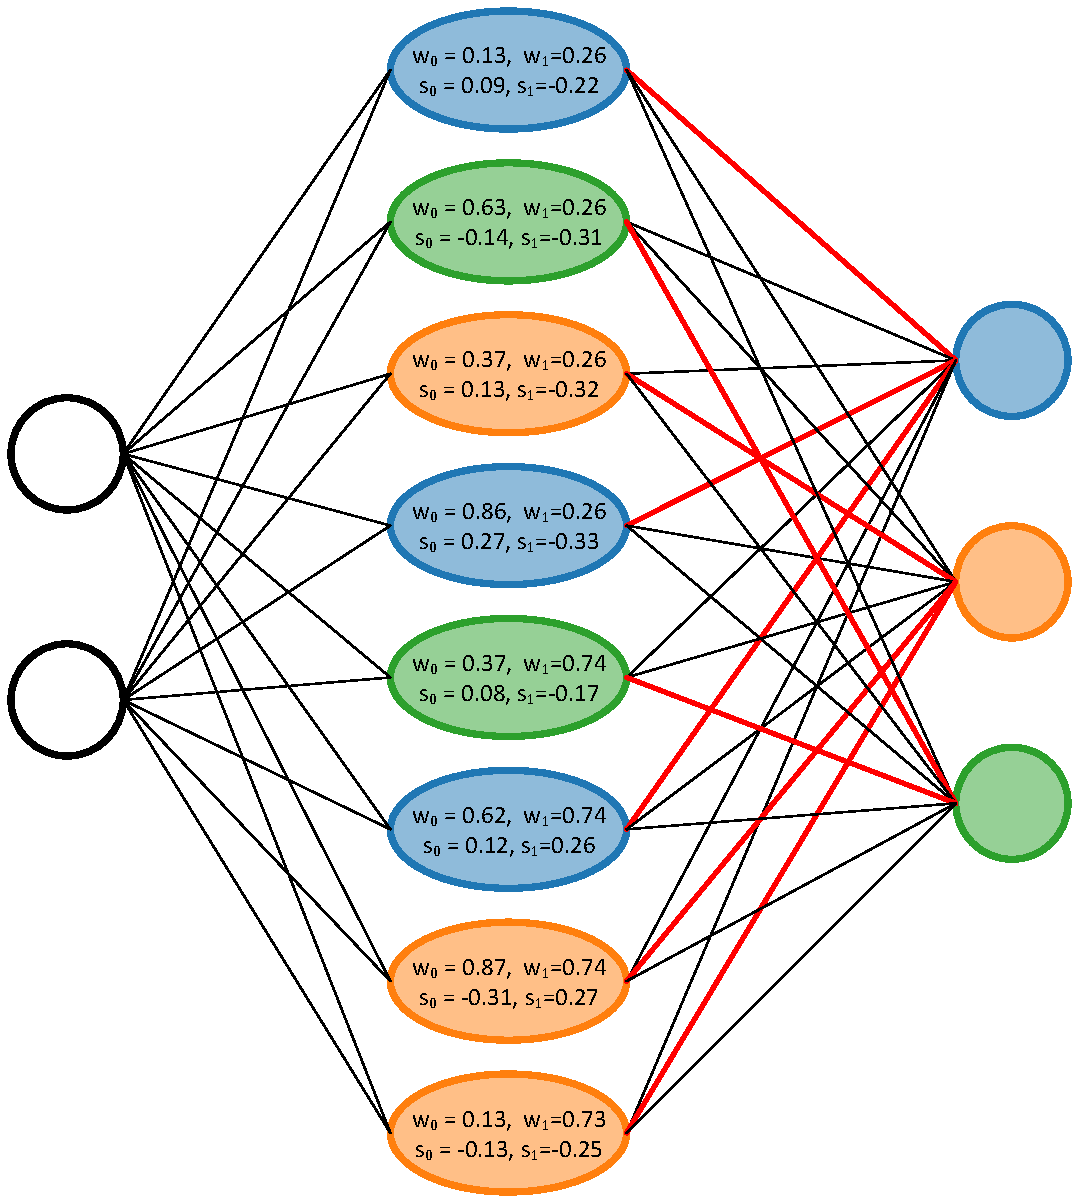
\includegraphics[width=0.9\textwidth]{img/neural2}
    \captionsetup{justification=centering}
    \caption{Težine neuronske mreže dobivene učenjem}
    \label{fig:zad4b}
\end{figure}
Zbog preglednosti na slici nisu prikazane težine zadnjeg sloja, zbog čega su navedene u tekstu.
Težine $1.$ neurona izlaznog sloja (označen plavom bojom):
\[-0.6650, 58.5970, -48.6333, -48.5189, 47.4685, -7.9635, 77.1416, -44.6683, -30.0705\]
Težine $2.$ neurona izlaznog sloja (označen narančastom bojom):
\[1.6031, -49.5050, -14.1830, 61.4077, -29.4708, -62.9745, -43.3601, 48.3917, 43.3171\]
Težine $3.$ neurona izlaznog sloja (označen zelenom bojom):
\[-0.7940, -33.5619, 66.6208, -32.8230, -16.5325, 84.0111, -21.6693, -46.1330, -10.6479\]
\pagebreak



\section*{5. zadatak}
Ova neuronska mreža je u manjem broju iteracija ostvarila zadanu pogrešku (brže je naučena). 
To je moguće objasniti većom ekspresivnošću mreže, zbog čega lakše dolazi do prenaučenosti.
Moguće je primjetiti kako centroidi više nisu nužno u središtima klasa, zbog čega se gubi mogućnost vizualizacije i interpretacije težina.
\begin{figure}[ht!] 
    \centering
    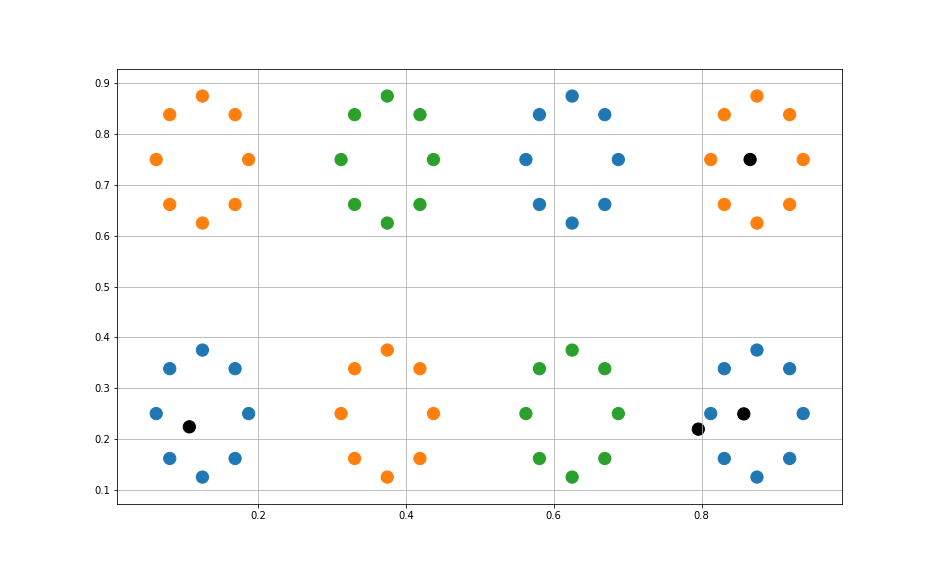
\includegraphics[width=0.9\textwidth]{img/zadatak5}
    \captionsetup{justification=centering}
    \caption{Centroidi dobiveni učenjem neuronske mreže arhitekture $2x8x4x3$}
    \label{fig:zad5}
\end{figure}
\pagebreak

\section*{6. zadatak}
Neuronska mreža manje arhitekture također može ostvariti zadano točnost te je na slikama \ref{fig:zad6a} i \ref{fig:zad6b} prikazano kako izgledaju centroidi dobiveni učenjem neuronskih mreža arhitekture $2x6x4x3$ odnosno $2x4x3$ koje obje postižu zadanu točnost. 
\begin{figure}[ht!] 
    \centering
    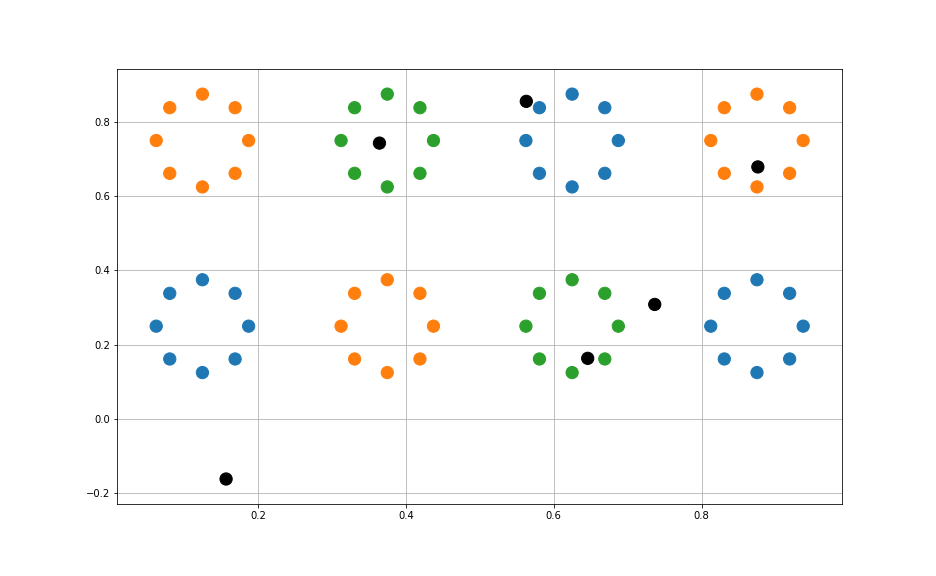
\includegraphics[width=0.9\textwidth]{img/zadatak6}
    \captionsetup{justification=centering}
    \caption{Centroidi dobiveni učenjem neuronske mreže arhitekture $2x6x4x3$}
    \label{fig:zad6a}
\end{figure}
\begin{figure}[ht!] 
    \centering
    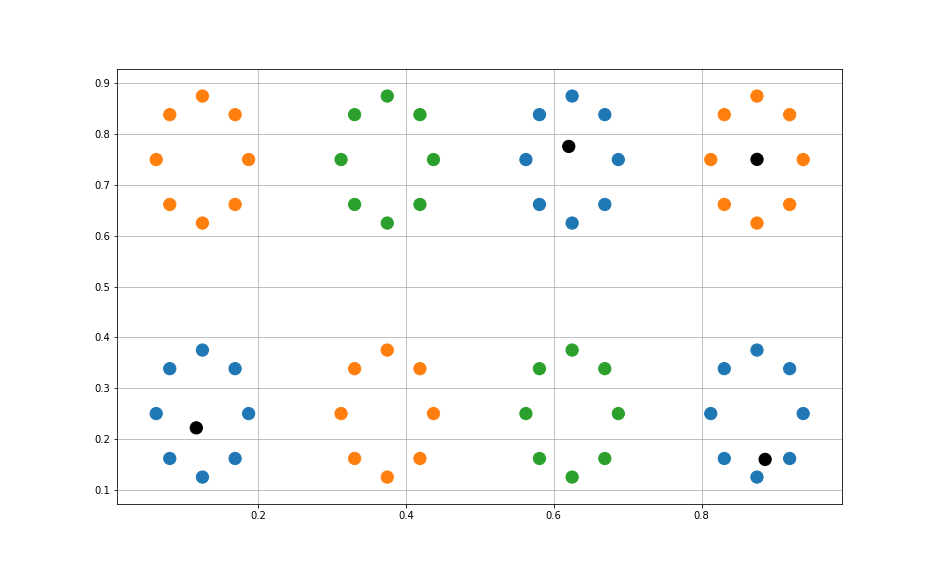
\includegraphics[width=0.9\textwidth]{img/2x4x3}
    \captionsetup{justification=centering}
    \caption{Centroidi dobiveni učenjem neuronske mreže arhitekture $2x4x3$}
    \label{fig:zad6b}
\end{figure}
\pagebreak
\end{document}